% äöüß
\chapter{p-Dopants in Amorphous Hosts}\label{chap:P-Doping}
\addcontentsline{lof}{chapter}{\thechapter\hspace*{1ex} p-Dopants in Amorphous Hosts}

\intro{%
After investigating n-doping in the last two chapters, this chapter investigates p-doped material systems. Two hosts and two dopants are chosen in order to study the influence of the molecular energy levels.
While the host material used for the n-doping experiments is the exceptionally well conducting polycrystalline \CS, the two hosts studied in this chapter are more typical amorphous \OSCs with approximately five orders of magnitude lower mobilities.
In \secref{ResP-Cond}, the conductivity of differently doped samples is studied. Afterwards, it is investigated how the \cLong is influenced by the temperature, which again supports a thermally activated hopping process and therefore allows to derive an \EactLong.
\Secref{ResP-S} presents thermoelectric (Seebeck) investigations for a variation of the temperature and the \CLong. The results are compared to the \EactLong and conclusions for the mobility are drawn. In \secref{ResP-Degradation}, the thermal stability is investigated and finally, in \secref{ResP-Conclusion}, the results are summarized.
}

\pagebreak

One major difference of p-doping to n-doping is that p-doped layers are usually degrading more slowly under air-exposure or under contact with residual quantities of O$_2$ present in the vacuum chamber. The reason is that oxygen leads to a p-doping as well\cite{Hamed1993} and hence to traps in n-doped layers.

Four different material combinations are investigated in this chapter. As host materials, \meo and \lili are chosen which have been both used in OLEDs\cite{Reineke2009} and OPV\cite{Maennig2004,HermenauRiedeLeo2012}. The host materials are selected to have slightly different \IEs, in particular \mbox{$\text{IE}=\eV{5.07}$} for \meo\cite{Tietze2012} and \eV{5.23} for \lili\cite{Meerheim2011}.
Two different p-dopants, \FS and \CSF, are studied, having estimated electron affinities of \mbox{$\text{EA}\approx\eV{5.00}$} for \FS\cite{Tietze2012,WellmannDiss} and \eV{5.38(30)} for \CSF\cite{Meerheim2011}. Since different techniques for the estimations have been used and the errors are rather large, the true values may differ.
From the measured values of the hosts' IEs and the estimated values of the dopants' EAs, the doping is expected to be more efficient for \CSF, whereas for \FS very low doping efficiency is expected.
However, energy levels are merely a rough guide to predict the doping effectiveness, as microscopic details like spatial arrangements of orbitals play an important role as well. While the two hosts are of similar weight, the dopant \CSF is almost 4~times as heavy as \FS.
Further details about the materials are summarized in the materials \secref{Mat}.

\section{Conductivity}\label{sec:ResP-Cond}
The first method of choice to study the doping is the investigation of the conductivity.
%
In comparison to the exceptionally well electron conducting \CS, used as host in the last two chapters, both investigated hole transporters are expected to show several orders of magnitude lower conductivities. This expectation is based on the fact that \CS molecules have a spherical shape and therefore align in an ordered face-centered cubic (fcc) polycrystalline structure\cite{Peimo1993} that allows for high charge carrier mobilities, whereas both hole transporting materials are expected to form amorphous layers with much lower mobilities, as discussed in \secref{MatMeO}.
OFET-mobility experiments\mphOFET yield similar carrier mobilities for both hole transport materials of \mob[2.3E-05] for \meo and \mob[5.7E-05] for \lili. These values are five orders of magnitude lower than record values for \CS\cite{Itaka2006}.

\subsection{Relation of Conductivity to Doping Concentration}%
\label{sec:ResP-CondMR}

\cBild
{MR-Cond-p-all-EvapVS30}
{As-prepared and post-annealed \cLong}
{Conductivity \c \vs \CLongL for samples of \meo (triangles) and \lili (squares) doped by \FS (empty symbols) and \CSF (filled symbols). (a) As-prepared, measured at \T[25]
and (b) after thermal annealing for 1~hour at \T[45] (\meo) or \grad{70} (\lili), probed at \T[30].
Dashed lines with slopes of 1.0, 1.5 and 2.5 are guides to the eye.
}

The conductivities of samples of \meo and \lili, doped by different \CLongs of \FS or \CSF are presented in \figref{MR-Cond-p-all-EvapVS30}\,(a), measured directly after sample fabrication at \T[25].
As a linear and symmetric current-voltage relation is detected for all samples, the contact resistance and consequently the injection are negligible. %
It can be seen that each dopant is able to dope both host materials, and the conductivity can be tuned over several orders of magnitude.

As discussed in the previous chapters, the samples are thermally annealed prior to further investigations, to ensure stable measurement conditions.
Only moderate temperatures are applied for samples of \meo, since is has a low glass transition temperature in the range of \Tg[67], as discussed in \secref{MatMeO}.
The samples are slowly heated from \T[25] to \grad{45} for \meo or to \grad{70} for \lili and kept at this temperature for 60~minutes. Afterwards, the samples are slowly cooled down and the measurement routine (compare \secref{ExpMeasRoutine}) starts with a conductivity experiment at \T[30]. This data, depicted in \figref{MR-Cond-p-all-EvapVS30}\,(b) shows that for most samples, the annealing has only minor influence on the conductivity.

% Observations
Samples of \meo doped by \FS yield the highest conductivity \c at each \CLong \C. A linear relation of $\c(\C)$ is found for low \C, whereas for \Cgr{0.030} up to the highest prepared \CLong of \C[0.290] a superlinear slope of 1.5 is determined, indicated by the dashed lines in \figref{MR-Cond-p-all-EvapVS30}. No saturation at high \CLongs is observed, in contrast to the n-doping experiments of chapters \ref{chap:PaddleWheels} and \ref{chap:AirStables}.
The highest measured conductivity is \c[1.73E-3] at \C[0.290]. Thermal annealing at \T[45] hardly has an influence on the samples of this material combination.

Doping \meo by \CSF instead, results for \Ckl{0.100} in the second highest conductivity value at each \CLong. At low \CLongs, a linear relation of $\c(\C)$ is found, indicated by the dashed line of slope 1.0, and at \Cgr{0.030} the slope is reduced. The highest detected conductivity is \c[8.31E-5] at \C[0.500]. Thermal annealing at \T[45] increases \c for most samples, only the lowest doped sample has a reduced value after annealing, despite measuring at \K{5} higher temperature.

\lili doped by \FS yields for \Ckl{0.100} lower conductivities than both \meo combinations. At \Cgr{0.060} a superlinear increase with a slope of 2.5 is determined without a saturation visible at high \CLongs. The highest detected conductivity is \c[1.44E-3] at \C[0.490], being close to the maximum measured for \meo doped by the same dopant, but at an almost twice as high \C. Thermal treatment reduces \c for weakly doped samples, whereas highly doped samples are almost unaffected.

Doping \lili by \CSF gives the lowest conductivities, with mostly one order of magnitude lower values compared to the same host doped by \FS. Starting from a value of $\c[2.2E-8]$ at \C[0.011], which is below the estimated resolution limit of the setup (compare \secref{ExpResLimit}), \c rises superlinearly with \C as well with a slope of 2.5 and reaches \c[6.10E-6] at \C[0.200]. Again, thermal treatment lowers the \c for weakly, but raises \c for highly doped samples.

Comparing the hosts, samples of \meo yield higher conductivities than samples of \lili for the same dopant. As for both hosts similar OFET-mobilities have been measured (\mob[2.3E-05] for \meo and \mob[5.7E-05] for \lili), the difference in \c must be due to the \nhLong \nh.
This finding is in agreement with \meo having a lower \IE than \lili (compare \secref{MatHosts}), which is expected to lead to \meo being easier to dope by p-dopants, and thus allowing for a higher doping efficiency. Both series that use \lili as host show the same strong slope of 2.5, indicating that either the doping efficiency or the mobility rises strongly upon increasing \CLong.

Comparing the dopants, it is found that for samples doped by the larger and 4~times heavier \CSF, the slope of the conductivity decreases at high \C, whereas for the lighter \FS instead the superlinear relation of $\c(\C)$ continues at high \C with no saturation in the investigated doping regime.
The absence of a saturation when doping by \FS is attributed to the fact that both hosts, \meo and \lili, form amorphous layers that are less sensitive to impurities than the polycrystalline \CS layers, investigated in the previous chapters \ref{chap:PaddleWheels} and \ref{chap:AirStables}.
The decreasing slope at high concentrations of \CSF is attributed to a disturbance of the microstructure by the heavy dopant, since at the same molecular doping ratio (MR), using \CSF leads to a 4~times higher dopant mass deposited into the layer.
Different slopes of $\c(\C)$ are discussed in detail in \secref{ResASCondMR} for \CS doped by \aob (linear) and \dmbi (superlinear). Here, for the \FS-doped samples, the trend is different, as for low \C a linear slope is found and only at high concentrations the slope increases. 
The thermal annealing effects the conductivity of samples doped by \CSF stronger than samples of \FS, suggesting that the thermal energy allows for rearrangement of the heavier molecules.

The conductivity data follows the opposite trend as expected from the energy levels given in literature.
Doping by \FS is more efficient than doping by \CSF for both hosts, which suggests that the roughly estimated EAs of the dopants are incorrect, since the measurements of the hosts IEs are more accurate.
As \FS is able to dope \lili (\mbox{$\text{IE}=\eV{5.23}$}) well the real EA of \FS is expected to be larger than this value. This statement is supported by the closely related dopant \FV having an \mbox{$\text{EA}=\eV{5.25}$}\cite{Gao2001}, measured by inverse photoemission spectroscopy (IPES). Cyclic voltammetry (CV) measurements on \FV and \FS yield similar values for the EA of both compounds\cite{WellmannDiss}, hence it is expected that the real EA of \FS is in the range of \mbox{$\text{EA}=\eV{5.25}$}, which is above the estimated literature value of \mbox{$\text{EA}\approx\eV{5.00}$}\cite{Tietze2012}.

As \CSF does not dope \lili with its \mbox{IE$=\eV{5.23}$} well, the real EA of \CSF is expected to be smaller than this value.
Furthermore, the saturation of \c at high \C of \CSF in both hosts indicates the EA of \CSF might even be smaller than or in the range of the IE of \meo (\mbox{IE$=\eV{5.07}$}).
%
Due to inter- and intra-molecular interactions, the IE and EA are no sharp levels but distributed in energy. Consequently, \CSF is able to dope some of the host molecules, despite its EA being expected to be low compared to the IE of both hosts. At high \C, most of the host molecules with sufficient small IE are already doped and additional dopants find no suitable hosts and the conductivity saturates. This model is supported by the data, since for \lili as host (with the larger IE) the saturation of \c occurs at lower \C than for \meo.

\subsection{Temperature Dependence of the Conductivity}%
\label{sec:ResP-CondEact}

\cBild{T-Cond-p}
{Temperature dependence of conductivity}
{Temperature dependence of the conductivity for four different material combinations. Lines are fits using \eqnrefPage{CondActivation}.
The contribution of the leakage current through the glass substrate is estimated for a \nm{30} thick layer using the data of \figrefPage{T-LeakCurrent}.
}

The conductivity increases with temperature for all samples, similar to the case of the n-doped samples discussed in the previous chapters. \Figref{T-Cond-p} presents the experimental data of all samples in Arrhenius plots.
Due to the low glass transition temperature of \meo (\Tg[67]), the samples with \meo as host material are only investigated in the range of \T[25] to \grad{45}, see \figref{T-Cond-p} parts (a) and (b). The samples comprising \lili on the other hand, are successfully investigated up to \T[70], some samples even up to \grad{80}, compare \figref{T-Cond-p} parts (c) and (d).
Since the detected temperature-dependent leakage currents through the glass substrate (as discussed in \secref{ExpLeakageCurrent}) are in a similar range to the measured currents, an estimation of their contribution to the conductivity of a \nm{30} thick layer at \V[1] is performed and included into \figref{T-Cond-p}.
It can be seen in \figref{T-Cond-p}\,(d) that for the three lowest doping concentrations of \CSF in \lili the contribution of the leakage currents cannot be neglected.

A linear relation of inverse temperature to conductivity is found in the Arrhenius plots. Therefore, again a thermally activated transport mechanism is concluded, allowing to derive an \EactLong \Eact via \eqnrefPage{CondActivation}. This property is plotted in \figref{MR-Eact-p-all} against the \CLong for all four material systems, excluding the three samples of the lowest doping concentrations of \CSF in \lili due to the relatively strong contribution of the leakage currents.

\cBild{MR-Eact-p-all}% passt leider nicht unter vorheriges
{Activation energy of the conductivity}%
{Activation energy of the conductivity \Eact, derived from the temperature dependence of the conductivity $\c(T)$ displayed in \figref{T-Cond-p}, calculated using \eqnrefPage{CondActivation} for
samples of \meo (triangles) and \lili (squares) doped by \FS (empty symbols) and \CSF (filled symbols).
}

The resulting values of the different samples range from \Eact[204] to \meV{374}, being much higher than observed for the n-doped samples of the previous chapters, where most values are found to be in the range of \Eact[50] to \meV{175}.
An almost linear reduction of \Eact with rising \CLong in this semi-logarithmic scale is present for all four material combinations, with no saturation visible.

Samples of \meo doped by \FS yield their largest value of \Eact[312] for the lowest used \CLong of \C[0.004]. This value is reduced to \Eact[211] at \C[0.290], corresponding to a linearly fitted reduction of $\meV{56}$ per order of magnitude of \C.

Doping \meo by \CSF instead, a value of \Eact[333] at the lowest \CLong of \mr{0.005} is reduced to \Eact[279] at \mr{0.500}. The slope of \meV{23} per order of magnitude is approximately half the value found for the \FS-doped samples.

For the combination of \lili doped by \FS, the largest \Eact[374] of all p-doped samples is detected at \C[0.010]. This material combination has the strongest change of \Eact showing a lowering of \meV{98} per order of magnitude of \C, as also the lowest value of all p-doped samples is reached by this combination with \Eact[204] at \C[0.490]. At low \CLongs, a smaller and at \Cgr{0.060} a larger slope is found. The \CLong of \mr{0.060} is the same from where on a superlinear gain in conductivity with \C is observed.

Doping \lili by \CSF, the \Eact[346] at \C[0.056] decreases to \meV{313} at \mr{0.200}, giving the highest values of all material combinations at the corresponding \CLong. The slope of the decrease derived from the three samples is \meV{60} per order of magnitude of \C.

In conclusion, the samples of all four material combinations yield the same tendency of a linear reduction of \Eact with increasing logarithm of \C. The samples with \meo as host material have smaller values of \Eact and smaller slopes compared to the \lili samples, in agreement with \lili having a larger IE. At low \C the curves are parallel, whereas at high \C for samples of \lili a faster decrease of \Eact is found.

Comparing the two dopants in each host material, similar values of \Eact are observed for low \CLongs of \FS and \CSF. With increasing \CLongs, the \Eact are diverging and the values obtained for using \CSF as dopant are higher compared to \FS.
At high \C, similar values for each dopant in both hosts are derived, with the samples doped by \FS approaching \Eact[200], being at least \meV{80} lower than for the highest \CSF-doped samples.
The larger \Eact for \CSF can be correlated to a thermal activation of dopant ionization. As discussed in \secref{ResP-CondMR} the conductivities of \CSF-doped samples saturate at high \C, indicating that the real EA of \CSF is smaller than the IEs of both hosts, \meo and \lili. In this case only a fraction of the \CSF molecules will be ionized. By rising the temperature, the number of ionized dopants increases due to more thermal energy, leading to an increase of the \nhLong \nh, which contributes to a higher conductivity at higher \T and thus raises \Eact. Additionally, a rise of \nh can also result in a gain of mobility\cite{Arkhipov2005,Arkhipov2005a}, further increasing the conductivity and hence \Eact.

In comparison to the n-doped \CS samples, discussed in the previous chapters, it can be seen that the \Eact of all p-doped samples are almost twice as high as the values derived for n-doped \CS samples at corresponding \CLongs. The values measured are also higher than literature values for instance the \Eact of VOPc\footnote{VOPc is vanadyl-phthalocyanine} p-doped by \FV range from \meV{280} to \meV{210} for low \CLongs of \C[0.002] to \mr{0.020}\cite{Pfeiffer1998}. The larger \Eact might be attributed to the amorphous hosts \meo and \lili, since \CS as well as VOPc form polycrystalline layers.
Similar to the findings for \CS using the air-stable n-dopants, \aob and \dmbi, an increase of \Eact at large \CLongs is not present.

% \newpage
\section{Thermoelectric Measurements}%
\label{sec:ResP-S}
\subsection{Temperature Dependence of the Seebeck Coefficient}
\label{sec:ResP-S-T}
%
%
\begin{figure}[p]
\centering%
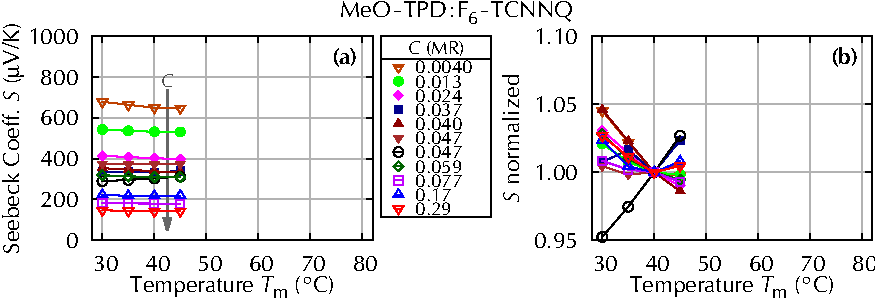
\includegraphics{plot/T-S-p1}\\%
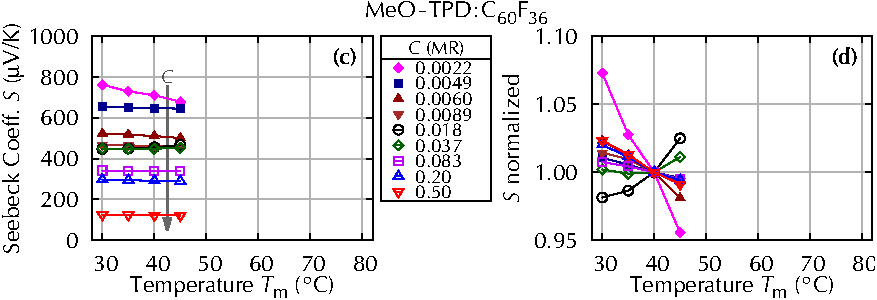
\includegraphics{plot/T-S-p2}\\%
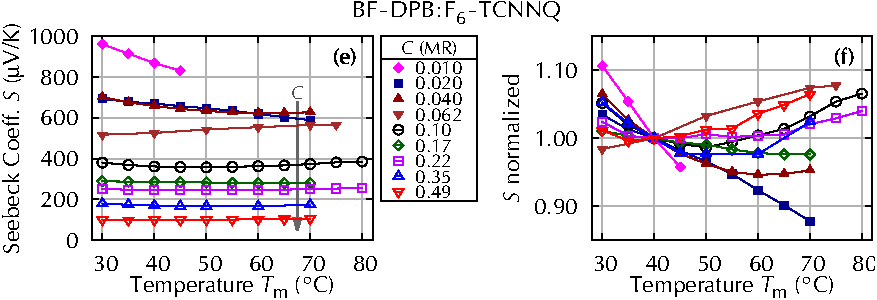
\includegraphics{plot/T-S-p3}\\%
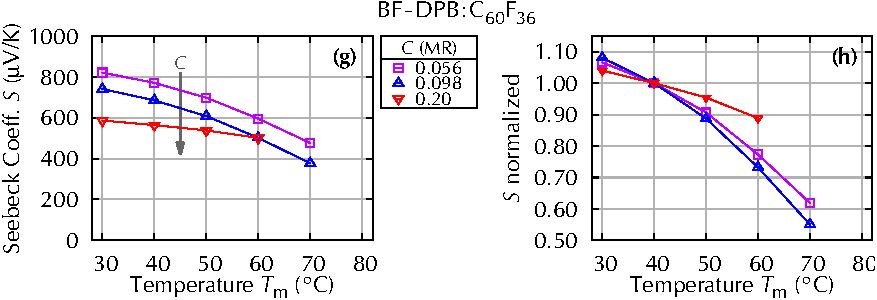
\includegraphics{plot/T-S-p4}\\%
\setcapwidth[c]{\tmCapWidth}%
\caption
[Temperature dependence of the Seebeck coefficient]%
{Temperature dependence of the Seebeck coefficient \S for four different material combinations,
left: absolute values,
right: normalized to the \Tm[40] measurements.
}%
\label{fig:T-S-p-all}
\end{figure}
%
%
Thermoelectric investigations at different temperatures are performed along with the conductivity experiments, similar to the studies of the n-doped samples. The resulting Seebeck coefficients \S at different temperatures are presented in \figref{T-S-p-all} for all four material combinations. As expected, all values of \S are positive in sign, thus holes are the dominating charge carrier species for all the p-doped samples. Electron conduction along the dopant molecules is not detected, not even for large \CLongs. The observed values for \S range from \uVK{100} to \uVK{1000} and a lowering of \S with rising \CLong is found. It was not possible to perform reliable Seebeck measurements on samples of \lili doped by \Ckl{0.030} of \CSF, as the resulting conductivities were below the resolution limit of the setup, as discussed in \secref{ExpResLimit}.

The samples with \meo as host material have only been measured in the range of \Tm[30] to \grad{45}, due to the low glass transition temperature of this material. Higher temperatures of up to \Tm[80] could be applied to the samples using \lili as host.
In order to investigate the influence of the temperature \Tm, the relative changes of \S, normalized to the value at \Tm[40], are depicted at the right hand side graphs in \figref{T-S-p-all}. A temperature of \grad{40} is chosen, as it is a device-relevant temperature and more stable to control than \Tm[30].

No clear trend of the temperature dependence of \S can be derived from the data. In the range of \Tm[30] to \grad{45} most samples vary by about $\pm5\,\%$.
This effect is much smaller than the influence a variation of the \CLong has.
The three samples of \lili doped by \CSF dramatically decrease in \S at elevated temperatures. This tendency is not present in the data of the other material combinations and is opposite to the results for n-doped \CS samples, where a gain of \S with temperature is found, as discussed in sections \ref{sec:ResPd-S-T} and \ref{sec:ResAS-S-T}. As a decreasing \S is correlated to an increasing \nhLong, the data of \lili doped by \CSF supports the theory of \CSF having a lower EA than the IEs of both hosts. Higher thermal energy allows to overcome the energetic difference and hence ionization of more and more dopants.

\subsection{Relation of Seebeck Coefficient to Doping Concentration}%
\label{sec:ResP-S-MR}
%
Comparing the Seebeck coefficients at one temperature of \Tm[40] for different \CLongs, a lowering of $\S$ with increasing \C is found for all four material combinations, ranging from \uVK{867} to \uVK{100}, as displayed in \figref{MR-See+Es-p-all}.
Using \eqnrefPage{S-Es-org}, the energetic difference \Es between the \EfLongL and the \EtLongL can be derived:
\begin{align}
 \Es =\S \cdot e \cdot \T \quad \text{ with } \quad\Es := \Ef - \Et
\PUNKT
\tag{\ref{eq:S-Es-org}}
\end{align}
\Es is given as the right hand axis in \figref{MR-See+Es-p-all}.
Following the trend of \S, the value of \Es decreases with increasing \C for both dopants, which is correlated to a shift of the \EfLong \Ef towards the \EtLong \Et. This finding is in agreement with the observations of the n-doped samples, where \Es drops with rising \CLong. No saturation is visible in the data and the samples of all four material combinations yield an almost linear relation of \S and \Es to the logarithm of \C.
%
\cBild[t]
{MR-See+Es-p-all}%
{Seebeck coefficient and derived \EsLong}
{Seebeck coefficient \S and derived \EsLongL at \Tm[40] for samples of \meo (triangles) and \lili (squares) doped by \FS (empty symbols) and \CSF (filled symbols).
}
%

The series of \meo doped by \FS starts at \C[0.004] with \Es[203]. This value is reduced to \Es[45] at \C[0.290], corresponding to a linear slope of \meV{88} per order of magnitude of \C.

Doping \meo by \CSF instead, a deviation from a linear relation is present between $\C[0.006]$ and \mr{0.018}. Overall the slope is determined to \Es[67] per order of magnitude of \C and therefore somewhat lower than for the use of \FS as dopant.

In case of \lili doped by \FS, the values for \Es at low \C are larger than observed for \meo as host material. At \Cgr{0.100} a reasonable agreement is found. The overall linear slope is \meV{142} per order of magnitude, being the highest of all four material combinations.

For the three reliably measurable samples of \lili doped by large concentrations of \CSF, the highest values of all four material combinations in the corresponding \C-regime are measured, with a maximum of \Es[241] at \C[0.056]. Here the slope is \meV{118} per order of magnitude of \C.

In conclusion, the samples of all four material combinations yield the same trend of a linear reduction of \S and \Es with increasing logarithm of \C.
Comparing the hosts, samples of \lili have larger values of \S and \Es and stronger slopes compared to samples of \meo. The larger values are in agreement with \lili having a larger IE than \meo, making electron transfer to the dopant less probable and therefore generating a lower \nhLong at the same \CLong for each dopant. This results in a greater energetic difference between \EfLong and \EtLong and thus a larger value of \S and \Es, particularly for doping by \CSF.
The strong slope of \S and thus \Es observed for \lili as host is attributed to filling of the tail states of the host's \dosLong that leads to a rapid shift of \Ef. At high \CLongs of \FS, a reduced slope is found, comparable to the samples of \meo.

Concerning the dopants, \FS leads to a lower value of \S and \Es and to a larger slope with \C than \CSF. The lower values of \S and \Es indicate a higher doping efficiency of \FS compared to \CSF. This finding supports the above proposed theory of \FS having a larger EA than \CSF, contrary to the literature values.

Comparing the results to the n-doped \CS samples of the previous chapters, larger values of \S and \Es are detected for the p-doped samples at low \CLongs.
This can be understood from the fact that the amorphous hosts investigated in this chapter are expected to have broader \dosLongs compared to the polycrystalline \CS. A broader host's \dos leads to a larger fraction of host molecules having a larger IE than the EA of the dopant and hence doping these molecules is less probable. Consequently, the \nhLong is lower which results in a larger \S and \Es.

\subsection{Comparison of Seebeck Energy and Activation Energy}
\label{sec:ResP-EsEact}

\cBild[b]{MR-Es+Eact-p}%
{Comparison of \Es and \Eact}
{Comparison of \EsLongL and \EactLongL for four different material combinations. \Es is probed at \Tm[40], \Eact is fitted from conductivity data presented in \figref{T-Cond-p}.}

In \figref{MR-Es+Eact-p}, \Es is compared to the previously discussed \EactLong \Eact, for the four different material combinations. All samples show an \Es that is approximately \meV{100} lower than \Eact. Such a large difference is not observed for the n-doped samples discussed in the previous chapters. In case of \CS n-doped by the air-sensitive dopants \CrPd and \WPd, a difference of only \meV{25} to \meV{75} is found at \Cgr{0.100}. That observation is attributed to a disturbance of the morphology by the large number of dopant molecules and hence a decreasing mobility with increasing \C, as discussed in \secref{ResPd-EsEact}.

\cBild[t]{MR-Eact-Es-p}%
{Difference between \Eact and \Es}
{Difference between \EactLongL and \EsLongL for samples of \meo (triangles) and \lili (squares) doped by \FS (empty symbols) and \CSF (filled symbols).
}

In order to investigate the difference of \Es and \Eact more closely, this quantity is plotted in \figref{MR-Eact-Es-p}.
Three of the four material combinations are in good agreement, only the three samples of \lili doped by \CSF show a difference that is smaller by $\approx\meV{50}$. The calculated differences range from \meV{100} to \meV{200} with one value as high as \meV{241}.
All material combinations yield a rising difference with \C at low \C.
Doping both hosts by \Cgr{0.050} of \FS, the difference between \Es and \Eact is found to be constant at a similar value around \meV{175}. This suggests that for all these samples the mobility has the same dependence on the temperature, compare \eqnrefPage{mob-von-Eact-Es-org}.

Samples doped by \CSF show a further increasing difference at larger \C, due to a faster decreasing \Es than \Eact at these \CLongs.
The slower drop of \Eact with \C at high \C of \CSF is attributed to thermal activation of dopants, due to the expected low EA of \CSF in respect with the IEs of the hosts as discussed in \secref{ResP-CondEact}. This model is supported by the temperature-dependent Seebeck experiments on the samples of \lili doped by \CSF, where a strong reduction of \S with increasing \T at high \C is observed, compare \figref{T-S-p-all}~(h).

\section{Degradation}\label{sec:ResP-Degradation}
%

In this section, the effect of elevated temperatures on p-doped layers is studied by conductivity investigations. Three samples of different material combinations are investigated. In order to compare the data, the conductivity of each sample is normalized to the value at \T[25], and depicted in \figref{killing-MeO}. The \cLong is measured twice with a delay of 30~minutes to 1~hour for most temperatures, which allows for detection of sample degradation. As reported in \secref{ResP-CondEact} for all samples at low \T, an increase of \c with \T is visible.

\cBild[t]
{killing-MeO}
{Degradation induced by heating}
{Degradation induced by heating for three different material combinations. The conductivity is normalized to the value at \T[25].}

The sample of \meo doped by \FS (at \C[0.040]) shows a slight degradation starting at \T[65]. A single measurement at \T[80] yields a maximum of \c, followed by a rapid decrease. The degradation is attributed to the glass transition of \meo (\Tg[67]\cite{Thelakkat1998}).

Doping \meo by \CSF (at \C[0.023]) a different tendency is found.
Between \T[70] and \grad{80} a sudden gain of \c by a factor of more than 3 is observed. 37~minutes later, at the same temperature, \c changes only by 1\,\%, so no degradation is visible at \T[80]. At \T[90] the sample is degrading rapidly. 
This data indicates that the presence of \CSF might shift the glass transition temperature of \meo upwards. Furthermore, it seems evident that thermal annealing raises the doping efficiency of \CSF in \meo.
As \CSF has been reported\cite{Mao2013} to thermally decompose at \T[120]\footnote{on indium tin oxide (ITO) substrates}, it is possible that in \meo the dopant decomposes as well. This could lead to a donation of strongly electronegative flour atoms to the host that would work as additional p-dopants and strongly increase the \nhLong.

Using \lili as host and \FS as dopant (at \C[0.100]), a higher thermal stability is found. Starting at $\T[65]$ a slow degradation of \c is observed, but up to \T[100] the effect is much lower than the gain due to the rising temperature. At $\T{}\geq\grad{115}$ a strong degradation is present.

No degradation is studied for \lili doped by \CSF.

\pagebreak
\section{Conclusion} \label{sec:ResP-Conclusion}
Comparing the host materials when using the same dopant, the samples of \meo show higher conductivities than samples of \lili, often by more than one order of magnitude. This trend is particularly interesting, as for both materials a similar OFET-mobility has been measured. Hence, the larger conductivity for \meo is attributed to a larger \nhLong due to the lower \IE compared to \lili.
The \EactLong is lower for \meo samples compared to \lili, but the difference decreases with increasing \CLong. A similar tendency is observed by the Seebeck investigations, showing that the Seebeck coefficients and hence \Es are larger for \lili, again with a decreasing difference with increasing \CLong.
These larger values obtained for \lili are in agreement with it having the larger IE, making electron transfer to the dopant less probable and therefore leading to a lower \nhLong compared to \meo. The strong slope of \S and hence \Es, observed for \lili as host is attributed to filling of tail states of the \dosLong.
Finally, it is evident that \lili has a higher thermal stability than \meo, which degrades already at \T[80].

Comparing the dopants in the same host material, higher conductivities are obtained for using the lighter \FS than for \CSF. This trend shows that \FS has a larger EA than \CSF, opposite to the estimated literature values\cite{Tietze2012,Meerheim2011}. For \FS, an EA larger and for \CSF an EA lower than \eV{5.2} is expected, as the IE of \lili is \eV{5.23} and only the former is able to dope it well.
The \EactLongs suggest a thermally induced ionization for large concentrations of \CSF, leading to higher \nhLong at elevated temperatures.
Seebeck measurements yield that in \meo, both dopants result in similar \S and hence \Es. At large \C, samples of \FS yield somewhat lower values compared to \CSF. In samples of \lili doped by \CSF much larger \S are found compared to doping by \FS. This suggests that \CSF generates a lower \nhLong in \lili, in agreement with its above discussed expected low EA. Temperature-dependent Seebeck studies show that for this material combination at elevated temperatures the resulting values of \S strongly decrease, supporting the model of thermal induced dopant ionization.

Most material combinations yield a strongly superlinear increase in \cLong with \CLong, opposite to the n-doping experiments of the previous chapters, where mostly linear relations are found.
Here, only for the combination of doping \meo by \CSF in the medium doping regime a linear relation is observed. In general, the host \lili and the dopant \FS lead to stronger slopes than the other materials.
%
While samples using \CSF yield a reduced slope at elevated \CLongs, samples doped by \FS continue to show strongly increasing \cLongs. Seebeck studies of samples doped by \FS show a rapid drop of the Seebeck coefficient in the medium doping regime indicating an increasing doping efficiency.
%
The comparison of conductivity and Seebeck investigations of samples of \meo doped by \CSF indicate that the decreasing slope of $\c(\C)$ at elevated \C is most likely due to a reduction of the mobility, since the Seebeck coefficient and hence the \nhLong is not saturating. This reduction is attributed to a disturbance of the layer morphology by the heavy dopant molecules. Analogously, the decreasing \c-slope of samples of \lili highly doped by \CSF is explained.

Overall, for devices the combination of the more stable host \lili with the stronger dopant \FS is advised.
In a future work the higher fluorinated compound C$_{60}$F$_{48}$ should be investigated, since it has been reported to have a larger EA than \CSF\cite{Liu1997} due to the increased amount of electron attracting fluorine atoms and has been shown to be electrically stable even upon twofold ionization\cite{Jin1994}.

